\section{Fundamentação Teórica}\label{sec:fund_teo}
\AtBeginSec

\begin{frame}{Canal de um Sistema de Comunicações Móveis}
 \begin{bigitem}
  \item O canal móvel sem fio apresenta muitos desafios, pois são muitos os fenômenos envolvidos na transmissão do sinal.
  \item Os principais efeitos que atrapalham o canal são:
  \begin{bigitem}
    \item Ruído.
    \item Desvanecimento de larga e pequena escala
  \end{bigitem}
 \end{bigitem}
\end{frame}


\begin{frame}{Critérios de Desempenho de um Sistema de Comunicações Móveis}
 \begin{bigitem}
  \item Ao desenvolver um sistema de comunicações, o objetivo é enviar o sinal ao usuário com eficiência e confiabilidade.
  \item Os recursos são limitados:
  \begin{bigitem}
    \item potência de transmissão;
    \item largura de banda;
    \item custo/complexidade envolvido para criar o sistema.
  \end{bigitem}
 \end{bigitem}
\end{frame}

\begin{frame}{Critérios de Desempenho de um Sistema de Comunicações Móveis}
 \begin{bigitem}
  \item Confiabilidade $\Rightarrow$ taxa de erro de bit (BER, \textit{Bit Error Rate}).
  \item O teorema da capacidade de informação de Shannon 
    \begin{equation}
     C = B\log_2\left(1 + SNR\right)\;\;bits/s
    \end{equation}
    onde B é larguda de banda do canal, SNR é a relação sinal-ruído e C é a capacidade de informação do canal, definida como a máxima taxa de informação que pode ser transmitida através de um canal sem erros, medida em bits/s.
 \end{bigitem}
\end{frame}

\begin{frame}{OFDM - Orthogonal Frequency Division Multiplexing}
 \begin{bigitem}
  \item OFDM é uma modulação de multiportadoras que transmite \textit{streams} de banda larga em canais paralelos de banda estreita, chamados de subportadoras.
  \item Vantagens:
    \begin{bigitem}
      \item Alta eficiência espectral.
      \item Fácil implementação.
      \item Resistência ao desvanecimento e interferência.
    \end{bigitem}
    \item Desvantagens:
    \begin{bigitem}
      \item Sensibilidade a deslocamentos de frequência.
      \item Problema PAR (\textit{Peak-to-Average Ratio})
    \end{bigitem}
 \end{bigitem}
\end{frame}

\begin{frame}{Comunicações Cooperativas}
 \begin{bigitem}
   \item Caminhos independentes entre o usuário e a ERB (Estação Rádio Base) são gerados através da introdução de um repetidor (\textit{relay}).
   \begin{figure}[!htb]
   \centering
   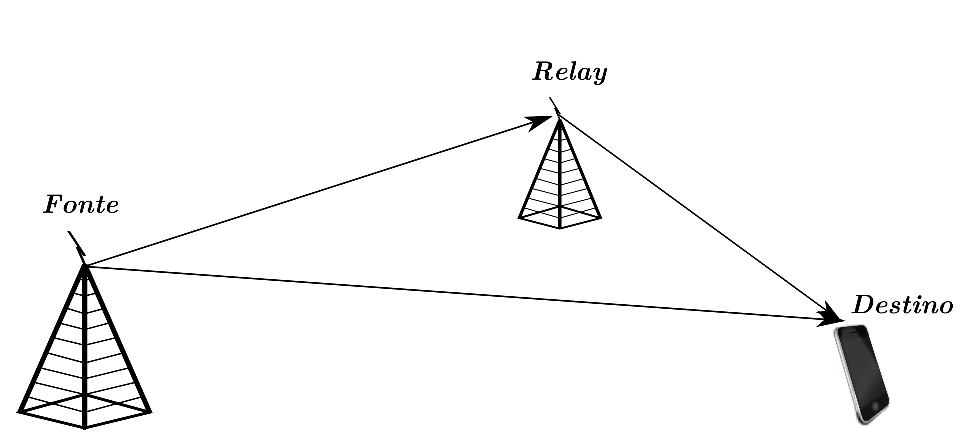
\includegraphics[width=0.60\linewidth]{../Imagens/relay_opt2.eps}
   \caption{Um modelo simplificado de comunicação cooperativa.}\label{fig:relay_ch}
  \end{figure}
 \end{bigitem}
\end{frame}


\begin{frame}{Comunicações Cooperativas}
  \begin{bigitem}
   \item Ao transmitir diversas cópias do sinal, é gerada diversidade espacial que pode ser explorada para combater os efeitos do desvanecimento.
   \item Existem duas principais estratégias de cooperação:
   \begin{bigitem}
      \item AF - Amplify and Forward.
      \item DF - Decode and Forward.
   \end{bigitem}  
  \end{bigitem}  
\end{frame}

\begin{frame}{Problemas de Otimização}
 \begin{bigitem} 
   \item Um problema de otimização padrão possui a forma:
   \begin{align}\label{eq:std_form}
       \min\quad &f_0(x)\\
        \text{suj:}\quad &f_i(x) \leq 0,\quad i=1,\ldots,m\\
                   &h_i(x) =0,\quad i=1,\ldots,p,
   \end{align}
   \item O vetor $x^*$ é dito uma solução do problema \eqref{eq:std_form}, se possuir o menor valor para a função objetivo dentre todos os vetores que satisfazem as restrições.
   \item Um problema de otimização convexa é aquele onde a função objetivo e funções de restrição são convexas, ou seja, satisfazem à inequação:
   \begin{gather}\label{eq:con_pro}
       f_i(\alpha x +\beta y) \leq \alpha f_i(x) + \beta f_i(y)\\
       \alpha + \beta = 1,\; \alpha \geq 0,\;\beta \geq 0.
   \end{gather}
 \end{bigitem}
\end{frame}

\begin{frame}{Alocação de Potência}
   \begin{bigitem}
      \item Um problema clássico em sistemas de comunicações é o da maximização da capacidade ou eficiência espectral em múltiplos canais paralelos
      \begin{figure}[!htb]
         \centering
         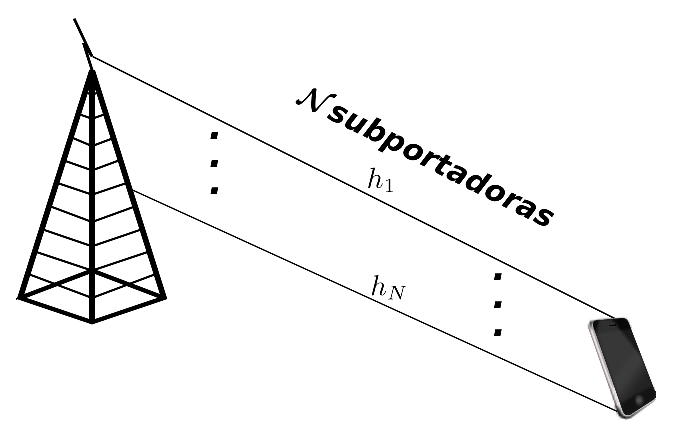
\includegraphics[width=0.50\linewidth]{../Imagens/cap_max_pr.eps}
%         \caption{Modelo de um sistema de canais paralelos OFDM.}\label{fig:cap_max_pr}
     \end{figure}
  \end{bigitem}
\end{frame}

\begin{frame}{Alocação de Potência}
\begin{bigitem}
   \item O problema recai em um problema de alocação de potência, onde deseja-se maximizar a taxa tendo como recurso escasso a potência de transmissão.
   \item Para o problema de otimização, é importante assumir:
   \begin{bigitem}
      \item O transmissor tem perfeito conhecimento das informações de coeficientes do canal.
      \item $N$ é o número de subportadoras, $h_n$ os coeficientes de ganho de canal associados com a subportadora $n$, $p_n$ é a potência do n-ésimo canal, $p_r$ é a potência do ruído e que a restrição total de potência do transmissor é 
      \begin{equation}\label{eq:pwr_cons}
         \sum_{n=1}^N p_n = p_t.
      \end{equation}
   \end{bigitem}
\end{bigitem}   
\end{frame}

\begin{frame}{Alocação de Potência}
   \begin{bigitem}
      \item O problema de otimização na forma padrão é escrito como
      \begin{subequations}\label{eq:cap_maxi}
        \begin{align}
          \min\quad & -C(p_1,\ldots,p_N) = -\sum_{n=1}^N \ln\left(1+\frac{p_n}{p_r}\|h_n\|^2\right)\label{seq:eff_esp}\\
            \text{suj:}\quad &\sum_{n=1}^N p_n = p_t\\
                            &-p_n \leq 0,\quad n=1,\ldots,N.
        \end{align}   
      \end{subequations}
      \item O problema é convexo e pode ser solucionado utilizando Otimização Convexa.
   \end{bigitem}
\end{frame}

\begin{frame}{Algoritmo Water-Filling}
   \begin{bigitem}
      \item Chamamos de \textit{water-filling} a solução para o problema \eqref{eq:cap_maxi}.
      \begin{figure}[!htb]
        \centering
        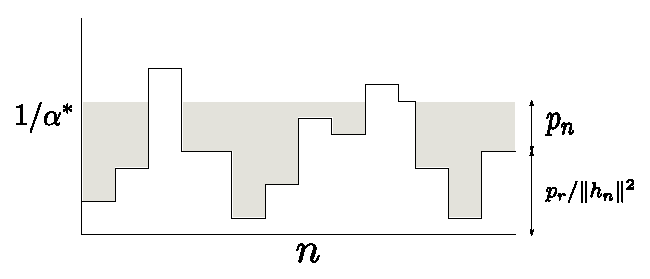
\includegraphics[width=0.80\linewidth]{../Imagens/water_filling.eps}
%        \caption{Ilustração do algoritmo \textit{Water-Filling}.}\label{fig:water_filling}
      \end{figure}
%      \item Pensamos em ${p_r}/{\|h_n\|^2}$ como o nível acima do solo para o trecho $n$, e então inundamos de água a região até a profundidade \(1/\alpha\).
   \end{bigitem}
\end{frame}

\begin{frame}{Algoritmo Water-Filling}
  \begin{bigitem}
     \item A solução pode ser escrita na forma de um algoritmo iterativo e com complexidade polinomial, chamado de \textit{water-filling}. 
     \item Primeiramente é feita a ordenação em ordem decrescente dos canais através de seus ganhos. 
     \item Através de no máximo $N$ iterações o algoritmo encontra a solução ótima para a potência de todas as subportadoras.
  \end{bigitem}
\end{frame}

\begin{frame}{Algoritmo Water-Filling}
   \begin{pseudocode}[ruled]{WaterFilling}{N,p_t,p_r,\mathbf{h}}
      \mathbf{p} \gets -1\\
      \WHILE p(N) < 0 \DO
      \BEGIN
        \lambda \gets N/(p_t + \sum_{n=1}^N p_r/h^2)\\
        \FOR n \GETS 0 \to N \DO
            p(n) \gets 1/{\lambda}-{p_r}{h(n)^2}\\
        \IF p(N) < 0
        \THEN
         N \gets N-1\\
      %   \END
        p(N) \gets 0
      \END\\
      \RETURN{\mathbf{p}}
   \end{pseudocode}
\end{frame}

